\section{Mô hình đề xuất}

% 2 slides:
% - Slide 1: Giới thiệu về ControlNet và LDM
% - Slide 2: Giới thiệu về mô hình huấn luyện và thực thi

\begin{frame}{Mô-đun Pseudo 3D (P3D)}

    \begin{columns}[c] 
        
        \begin{column}{0.55\textwidth}
            Phân rã nhân tích chập 3D ($d \times k \times k$) thành 2 thành phần nối tiếp:
            \begin{itemize}
                \item Nhân không gian (S): $(1 \times k \times k)$
                \item Nhân thời gian (T): $(d \times 1 \times 1)$ 
            \end{itemize}
            Thực hiện tuần tự, không đồng thời.
        \end{column}
        
        \begin{column}{0.3\textwidth}
            \centering
            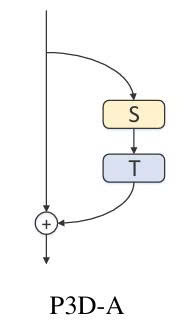
\includegraphics[width=\linewidth]{Figures/p3d_a.jpg}
        \end{column}
        
    \end{columns}

    \vspace{0.2cm}
    
    Mô-đun P3D đã giúp giảm độ phức tạp tính toán khoảng 2.25 lần so với kỹ thuật ARME đã dùng trước đó, giúp tăng tốc độ suy luận của hệ thống.

\end{frame}


\begin{frame}{Mô hình khuếch tán trong không gian tiềm ẩn}

\begin{figure}
    \centering
    
\includegraphics[width=0.9\linewidth]{Figures/LDM_arch.png}
     % \caption{Kiến trúc mô hình khuếch tán trong không gian tiềm ẩn}
\end{figure}

Sử dụng mô hình tiền huấn luyện Stable Diffusion được huấn luyện trên 2 tỉ cặp ảnh và văn bản của tập dữ liệu LAION.

\end{frame}

\begin{frame}{Mô hình đề xuất}

    \begin{figure}
        \centering
        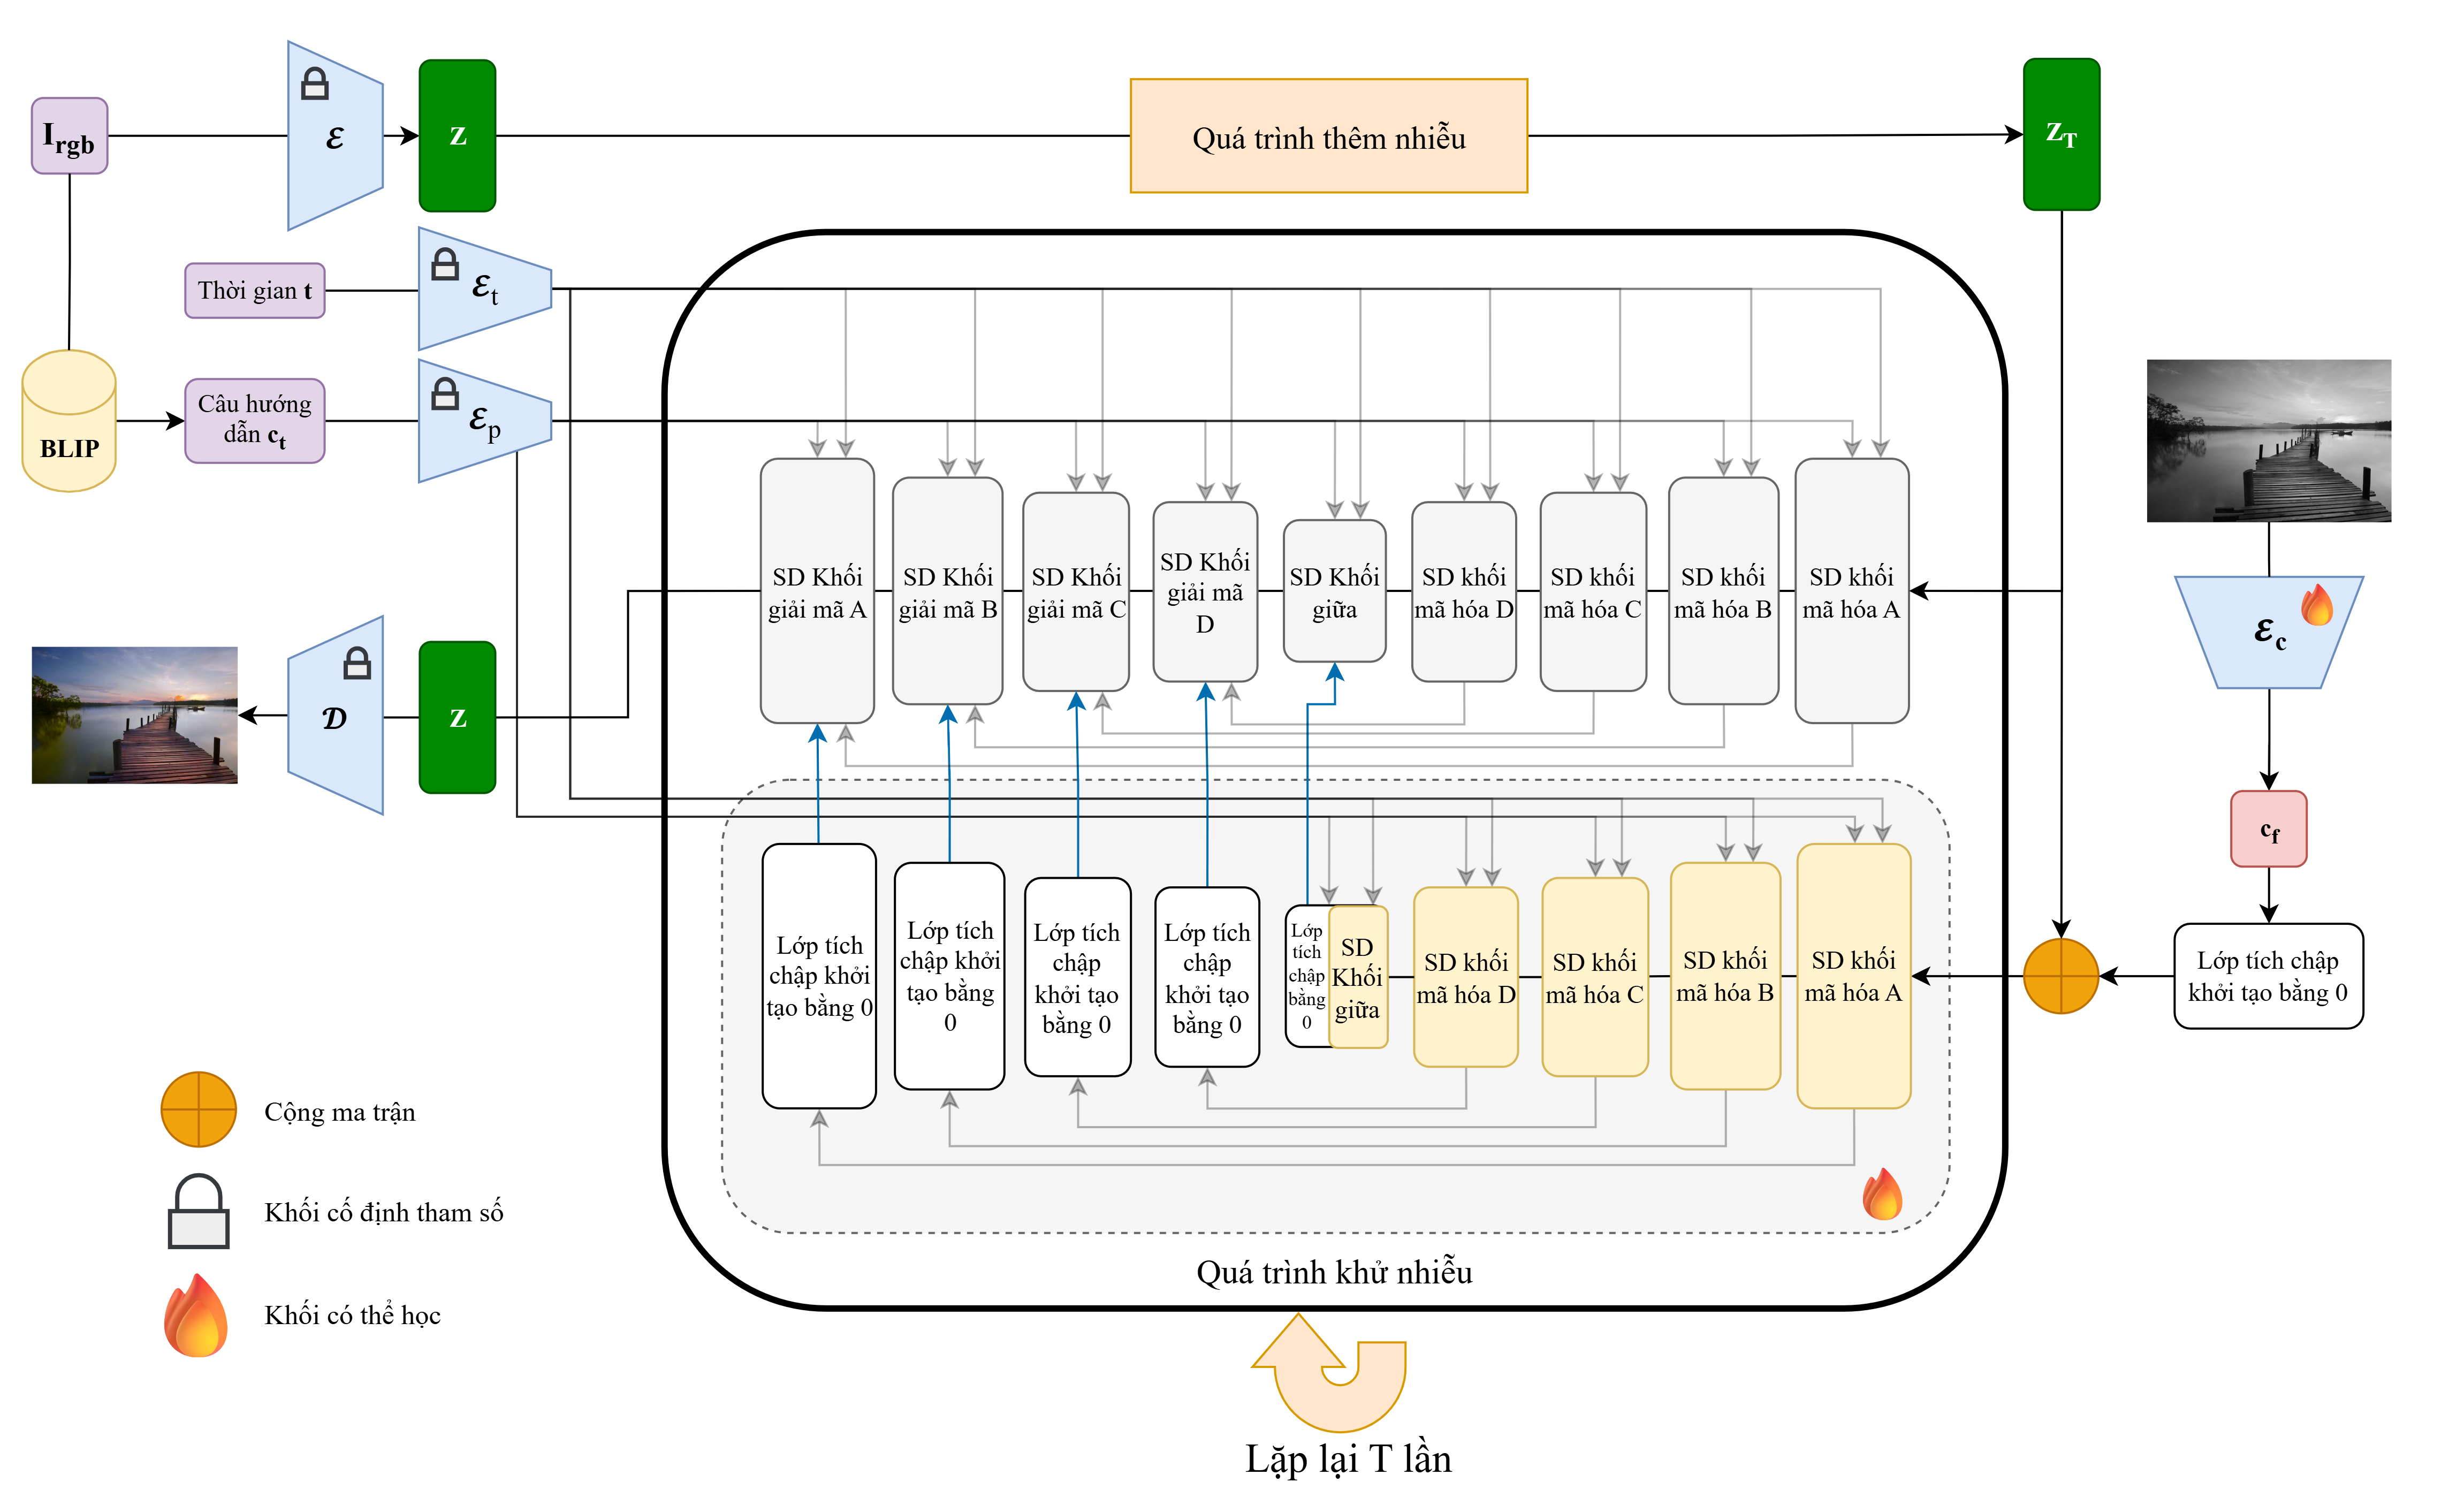
\includegraphics[width=0.9\linewidth]{Figures/main_model.png}
        % \caption{Kiến trúc mô hình đề xuất}
    \end{figure}


   
\end{frame}